% !TeX program = xelatex
% IEEE conference-format research proposal (revised, v2).
% Every typed number carries a "% src:" comment naming the file it comes from (paths relative to the repo root).
\RequirePackage[T1]{fontenc}
\documentclass[conference]{IEEEtran}

\usepackage{fontspec}
% Times/Helvetica/Courier-compatible fonts available in TeX Live and Overleaf.
\setmainfont{TeX Gyre Termes}
\setsansfont{TeX Gyre Heros}
\setmonofont{TeX Gyre Cursor}
\usepackage{cite}
\usepackage{amsmath,amssymb}
\usepackage{booktabs}
\usepackage{graphicx}
\usepackage{balance}
\usepackage{xurl}
\usepackage{tabularx}
\usepackage{array}
\usepackage{multirow}
\usepackage{tikz}
\usetikzlibrary{positioning,arrows.meta}
\usepackage[hidelinks]{hyperref}
\urlstyle{tt}
\hypersetup{
    pdfauthor={Yu Zhang and MingDong Wu and Zhixiong Zhang and Zhihao Tang},
    pdftitle={Near-LLM Quality at Decision-Model Speed? Comparing LLM-Based Approaches for C/C++ Memory-Leak Detection on a Debiased Juliet: Revised Project Proposal}
}

% Keep four full author blocks in two centered rows.
\makeatletter
\newcommand{\linebreakand}{%
    \end{@IEEEauthorhalign}
    \hfill\mbox{}\par
    \mbox{}\hfill\begin{@IEEEauthorhalign}
}
\makeatother

% Notation shared with the final paper (report/final_en/main.tex).
\newcommand{\Orig}{\textsc{Orig}}
\newcommand{\Deb}{\textsc{Debiased}}
\newcommand{\Dead}{\textsc{DeadFree}}
\newcommand{\Plac}{\textsc{Placebo}}
\newcommand{\code}[1]{\texttt{#1}}
\newcommand{\cwe}{CWE-401}

\title{Near-LLM Quality at Decision-Model Speed?\\
Comparing LLM-Based Approaches for C/C++ Memory-Leak Detection on a Debiased Juliet\\[0.3em]
\large Revised Project Proposal}
\author{
\IEEEauthorblockN{Yu Zhang}
\IEEEauthorblockA{ShanghaiTech University\\
Shanghai, China\\
\href{mailto:Zhangyu12026@shanghaitech.edu.cn}{Zhangyu12026@shanghaitech.edu.cn}}
\and
\IEEEauthorblockN{MingDong Wu}
\IEEEauthorblockA{ShanghaiTech University\\
Shanghai, China\\
\href{mailto:wumd2024@shanghaitech.edu.cn}{wumd2024@shanghaitech.edu.cn}}
\linebreakand
\IEEEauthorblockN{Zhixiong Zhang}
\IEEEauthorblockA{ShanghaiTech University\\
Shanghai, China\\
\href{mailto:zhangzhx2026@shanghaitech.edu.cn}{zhangzhx2026@shanghaitech.edu.cn}}
\and
\IEEEauthorblockN{Zhihao Tang}
\IEEEauthorblockA{ShanghaiTech University\\
Shanghai, China\\
\href{mailto:tangzhh2026@shanghaitech.edu.cn}{tangzhh2026@shanghaitech.edu.cn}}
}

\begin{document}
\maketitle

\begin{abstract}
We propose a controlled comparison of memory-leak detectors on the C/C++ \cwe{} cases of the Juliet~1.3 test suite.
The detectors fall into three families: classic program analysis, prompted large language models (LLMs), and \emph{decision models}, which return a label in a single forward pass.
A pilot audit shows that the original Juliet units can be classified without reading the memory logic.
Every good entry is declared \code{static void}, and a one-line ``no \code{free}/\code{delete} means leak'' rule already reaches macro-F1~0.935. % src: juliet_full/data/build/probes_report.md (grep v0, original, eval)
We therefore rebuild the benchmark.
\Deb{} has one good entry per test group, no \code{static} or wrapper cue, renamed identifiers, and labels checked by compilation and LeakSanitizer.
\Dead{} adds frees that are never executed, and \Plac{} applies the same edit with a harmless statement as a control.
The primary comparison axis is the prompting strategy (L1~Direct, L2~Few-shot, L3~Analysis-guided, L4~Neuro-symbolic) on two LLMs.
The secondary axis compares detector families: four static analyzers, a learned baseline, three decision models, and a grep rule.
We report accuracy with clustered confidence intervals, together with latency and cost for IDE, pre-commit, and CI use.
We also report robustness to never-executed frees, adjusted with the placebo.
This revision replaces our original SecVulEval-based proposal; the reasons are given in Section~\ref{sec:revision}.
\end{abstract}

\begin{IEEEkeywords}
memory leak, CWE-401, Juliet test suite, static analysis, large language models, benchmark validity
\end{IEEEkeywords}

\section{Introduction and Motivation}
\label{sec:intro}
A memory leak (\cwe{}, ``missing release of memory after effective lifetime''~\cite{mitrecwe401}) happens when a program allocates memory and loses its last reference before releasing it.
In C and C++ the programmer is responsible for releasing heap memory.
A leaking path may run only under rare conditions, such as a particular branch or a failed \code{realloc}, so leaks often survive testing.
Detecting them is a classic task for program analysis.
Path-sensitive analyzers track allocations along feasible paths.
Examples are the Clang Static Analyzer~\cite{clangsa}, Infer and its Pulse engine~\cite{calcagno2015infer,le2022pulse}, CodeQL~\cite{codeqldocs}, and Cppcheck~\cite{cppcheck}.
Dynamic tools such as AddressSanitizer/LeakSanitizer~\cite{serebryany2012asan,lsan} and Valgrind~\cite{nethercote2007valgrind} report leaks on executed paths only.

Two newer families of detectors now compete with these tools.
The first is the \emph{prompted LLM}.
An LLM can read a function and answer ``leak'' or ``no leak''.
It can also take analyzer warnings as extra input~\cite{wen2024llm4sa}, or produce facts that a symbolic engine then evaluates~\cite{wang2024nesa,wang2024llmdfa}.
The second is the \emph{decision model}.
Such a model returns a constrained label in one forward pass rather than generating free text.
Examples are hosted ``System One'' models such as Jev~\cite{typesafejev}, Intern-Decision~\cite{zhu2026interndecision}, and small LoRA-tuned~\cite{hu2022lora} classifiers trained with matched contrastive objectives~\cite{zhao2026cyberjev}.
These families have very different costs, from milliseconds on a laptop CPU to API calls priced per token.
They also differ in their failure modes.
This course is about AI for program analysis, and so we ask a direct question.
On the same units and under the same scoring, how do LLM-based detectors compare with established analyzers, and do they read the memory logic or only the surface of the code?

The second half of that question matters because benchmark artifacts can inflate learned detectors~\cite{risse2024limits,risse2025topscore}.
Juliet is widely used for this task~\cite{boland2012juliet,black2018juliet13}.
It is generated from templates, and its good and bad variants differ in systematic, non-semantic ways~\cite{germano2025biased}.
Our pilot audit (Section~\ref{sec:data}) confirms these artifacts for \cwe{} and makes them measurable.
The project therefore has two parts.
First, we rebuild a debiased, label-verified \cwe{} benchmark with a stress layer and a placebo control.
Second, we use it to compare more than 20 detector configurations. % src: report/final_en/OUTLINE.md (contribution "20+ detector configurations")
For each configuration we measure accuracy, latency, cost, and robustness.

\section{Revision Note: What Changed and Why}
\label{sec:revision}
\textbf{Original plan.}
The original proposal studied function-level vulnerability detection and vulnerable--fixed pair discrimination on SecVulEval~\cite{ahmed2026secvuleval}.
Memory leaks were only one category among many.
\textbf{Why we pivoted.}
We had three reasons.
\begin{enumerate}
\item Our frozen SecVulEval subsets contained only 4 \cwe{} vulnerable functions (2 of 160 in the detection subset and 2 of 200 pairs). % src: research/cwe401_scope.md:3
This is too few for any \cwe{}-specific conclusion.
\item Build-dependent analyzers could not run on isolated real-world functions. In a pilot, \code{clang -fsyntax-only} accepted 0 of 20 functions, because headers, macros, and type definitions were missing. % src: research/evaluation_protocol.md:30
Without them, the course's ``analysis-guided'' strategy and every static baseline would be impossible.
\item The course guide's example design fits a compilable synthetic suite: Juliet, a frozen dev/test split, and L1~Direct, L2~Few-shot, and L3~Analysis-guided prompting.
\end{enumerate}
\textbf{What we keep.}
We keep the methodological core of the original proposal:
(i)~a primary comparison axis that is fixed before any test run;
(ii)~frozen, hashed splits in which the development set alone is used to tune prompts and thresholds;
(iii)~leakage controls on model inputs (no label-revealing identifiers, comments, or strings);
(iv)~cost accounting from recorded token usage plus a common price card;
(v)~a strict scoring view in which a failed call counts as wrong and coverage is reported;
(vi)~clustered bootstrap intervals and paired McNemar tests with multiplicity correction.
\textbf{What moves.}
The SecVulEval pilot is no longer part of the evaluation. It will appear as an appendix of the final paper, where it documents why the pivot was needed.

\section{Research Questions}
\label{sec:rq}
\noindent\textbf{RQ1 (benchmark validity).} Can the original Juliet \cwe{} units be classified from format shortcuts alone, and does \Deb{} remove these shortcuts while keeping labels correct?

\noindent\textbf{RQ2 (approaches).} On \Deb{}, how do the prompting strategies L1--L4 compare on DeepSeek-V4.1-Flash and Qwen3.5-4B? How do decision models (Jev, Intern-Decision-4B, our LoRA decision model) and static analyzers compare with them?

\noindent\textbf{RQ3 (efficiency).} What are the accuracy--latency--cost trade-offs, and which detectors fit the latency budgets of an IDE, a pre-commit hook, a CI pull-request check, or a nightly scan?

\noindent\textbf{RQ4 (robustness).} How much does each detector change when frees that are never executed are inserted (\Dead{}), after we subtract the effect of the same edit with a harmless statement (\Plac{})? Does fine-tuning increase reliance on the presence of a \code{free}?

\textbf{Comparison axes.}
As the course guide requires, the \emph{primary axis} is the prompting strategy (L1--L4) applied to two LLMs of very different scale, one hosted and one local.
We fixed this axis and the pre-registered tests (Section~\ref{sec:eval}) before running on the evaluation split.
The \emph{secondary axis} is the detector family: static analyzers, prompted LLMs, decision models, a learned baseline, and a trivial rule.
Dynamic tools serve as a reference oracle and are not ranked.

\section{Dataset}
\label{sec:data}
\subsection{Source and unit of analysis}
We use every \cwe{} test case of Juliet C/C++~1.3~\cite{sardjuliet13,black2018juliet13}.
They form 1,658 test groups from 42 functional families and 48 flow variants. % src: juliet/full_split_v1.json (groups, family, variant counts)
Of the groups, 868 are C and 790 are C++. % src: juliet/full_split_v1.json (language)
By leak mechanism, 960 are \code{malloc}/\code{calloc}-style allocations, 588 are C++ \code{new}, 108 are \code{realloc} failures, and 2 are destructors. % src: juliet/full_split_v1.json (mechanism)
A \emph{unit} is one entry function together with its source/sink helpers.
The task is binary: \emph{leak} or \emph{no leak}.
Each group yields one bad unit and one good unit, so the benchmark has 3,316 units, half of them leaks. % src: juliet_full/data/README.md (layer1.jsonl 3,316 units)

\subsection{Pilot audit: format shortcuts in \Orig}
In the original Juliet files (\Orig{}), a bad unit is a single \code{bad()} function.
A good unit is a set of \code{static void goodG2B()}/\code{goodB2G()} functions plus a \code{good()} wrapper.
We fitted trivial probes on the dev split and scored them on the 2,656 evaluation units. % src: juliet_full/data/build/probes_report.md (eval 2,656 units)
The token \code{static void} appears in 100.0\% of good units and 0.0\% of bad units, so a rule that tests for it reaches macro-F1~1.000. % src: juliet_full/data/build/probes_report.md
A function-count rule reaches 0.924. % src: juliet_full/data/build/probes_report.md
The grep rule ``no \code{free}/\code{delete} means leak'' reaches 0.935. % src: juliet_full/data/build/probes_report.md (grep v0, original)
A bag-of-words logistic regression reaches 1.000. % src: juliet_full/data/build/probes_report.md (BoW LR, original)
Germano et al.\ report the same kind of bias for LLM-based detection on Juliet~\cite{germano2025biased}.
Accuracy on \Orig{} therefore says little about whether a detector understands ownership and release.

\subsection{Construction of \Deb{}}
Each unit of \Deb{} is a compilable program together with the model-visible text.
\begin{itemize}
\item \emph{One good entry per group.} We keep a single good entry, either G2B (good source, bad sink: the buffer lives on the stack) or B2G (bad source, good sink: the heap buffer is freed in the sink). The choice uses a fixed seed and is stratified by split, flow category, and mechanism, so that each stratum is half G2B and half B2G. % src: juliet_full/data/README.md
The groups in the \code{realloc}-failure and destructor families (110 groups) have no G2B/B2G split and use their \code{good1}/\code{good2} entries instead. % src: juliet_full/data/README.md
\item \emph{Shortcut removal.} We remove \code{static} from all function definitions, drop the \code{good()} wrapper, rename the entry function to \code{sym\_0}, and give bad and good units an identical driver \code{main}.
\item \emph{Cleaning.} We remove comments and the \code{OMITBAD}/\code{OMITGOOD} macros, inline the needed headers, and rename every identifier that contains \code{bad}, \code{good}, or \code{cwe}. An automated leakage test checks that no identifier, comment, or string matches \code{bad|good|g2b|b2g|cwe|leak|omit|flaw|fix}. All 6,632 records pass. % src: juliet_full/data/README.md
\item \emph{Label verification.} All 3,316 units compile under both gcc and clang~23. % src: juliet_full/data/build/verify_report.md
We run every unit under AddressSanitizer with LeakSanitizer (\code{use\_stacks=0}). LSan finds no leak in any of the 1,658 good units. % src: juliet_full/data/build/verify_report.md
It reports a leak in 1,474 of the 1,658 bad units (914+558+2). % src: juliet_full/data/build/verify_report.md (c_alloc 914, cpp_new 558, destructor 2)
Each of the 184 remaining bad units has a documented cause: 108 need a \code{realloc} failure, 68 keep the memory reachable from a global at exit, and 8 belong to variant~12, whose branch is random. % src: juliet_full/data/build/verify_report.md (mismatch reasons)
We therefore keep the Juliet label and record these causes. We treat dynamic tools as a reference and do not use them to define labels.
\end{itemize}
The same probes collapse on \Deb{}. The \code{static void} rule falls to 0.333, the function-count rule to 0.499, and the grep rule to 0.701. % src: juliet_full/data/build/probes_report.md (layer1)
The grep rule still scores 0.959 on B2G units but only 0.354 on G2B units. % src: juliet_full/data/build/probes_report.md (grep v0 layer1 B2G/G2B)
This split is expected: in a G2B unit, the good version has no \code{free} at all.
Every format-probe score is at most 0.60, the acceptance threshold we set in advance (PLAN.md~\S2.6). % src: juliet_full/data/build/probes_report.md (acceptance: format probes <= 0.60 PASS)

\subsection{Stress layer \Dead{} and control \Plac{}}
\Dead{} tests whether a detector treats ``a \code{free} is present'' as ``no leak''.
Into every unit, bad and good alike, we insert a free in a guard that is never true: \code{free} in C, and the matching \code{delete} or \code{delete[]} in C++.
We also wrap the real frees of good units in guards that are always true.
Every guard compares a file-local constant (\code{static const int sym\_N = V;}).
Each of six comparison forms is used in both a true and a false version.
Within each pair, the bad and the good unit have the same number of free statements and the same number of guards. % src: juliet_full/data/README.md (stress layer)
\Plac{} performs the same insertions with a harmless \code{printLine(...)} statement and leaves the real frees unwrapped.
It therefore separates the effect of a dead \emph{free} from the effect of editing the code at all.
We verify both layers again. All 3,316 units compile, and the LSan verdict matches stage~1 for 3,303 \Dead{} and 3,307 \Plac{} units. Every difference is in the random variant~12. % src: juliet_full/data/build/verify_layer3_report.md
On \Dead{}, the grep rule falls to 0.333. % src: juliet_full/data/build/probes_layer3_report.md (grep v0 layer3)

\subsection{Frozen split}
We split by \emph{flow variant} rather than by file.
The development and evaluation sets therefore never share a control-flow template.
The split is stored in \code{juliet/full\_split\_v1.json} (seed 20261123; SHA-256 prefix \code{08017a6f}). % src: juliet/full_split_v1.json (seed); sha256sum juliet/full_split_v1.json
The development set contains 9 variants (04, 10, 17, 18, 31, 41, 65, 68, 73). % src: juliet/full_split_v1.json (dev_variants)
We use it only to choose prompts and few-shot examples, to select checkpoints, and to set thresholds.
Variants 01 and 12 must stay in the evaluation set. % src: juliet/full_split_v1.json (rules.keep_in_eval)
The evaluation set contains the other 39 variants, divided into three folds by variant (Table~\ref{tab:split}). % src: juliet/full_split_v1.json (fold_variants 15/12/12)
Trained models are evaluated with 3-fold grouped cross-validation. Each fold is predicted by a model trained on the other two folds, and the dev set serves only for validation.

\begin{table}[t]
\centering
\caption{Frozen split \code{full\_split\_v1}. A unit is one bad or one good entry, so units $=2\times$ groups.}
\label{tab:split}
\setlength{\tabcolsep}{4.5pt}
\begin{tabular}{@{}lrrrrr@{}}
\toprule
Split & Variants & Groups & Units & C / C++ groups & \code{realloc} fail \\
\midrule
Dev        &  9 &   330 &   660 & 184 / 146 & 24 \\ % src: juliet/full_split_v1.json (summary.dev)
Eval       & 39 & 1,328 & 2,656 & 684 / 644 & 84 \\ % src: juliet/full_split_v1.json (summary.eval)
\quad fold 0 & 15 & 472 & 944 & 250 / 222 & 30 \\ % src: juliet/full_split_v1.json (summary.fold_0, fold_variants)
\quad fold 1 & 12 & 424 & 848 & 230 / 194 & 30 \\ % src: juliet/full_split_v1.json (summary.fold_1, fold_variants)
\quad fold 2 & 12 & 432 & 864 & 204 / 228 & 24 \\ % src: juliet/full_split_v1.json (summary.fold_2, fold_variants)
\midrule
Total      & 48 & 1,658 & 3,316 & 868 / 790 & 108 \\ % src: juliet/full_split_v1.json
\bottomrule
\end{tabular}
\end{table}

\begin{figure}[t]
\centering
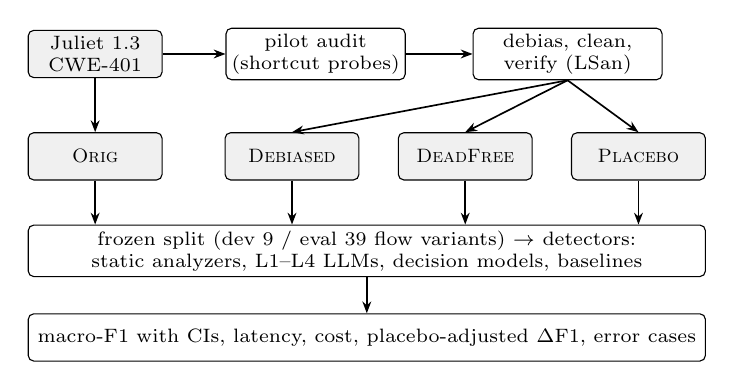
\begin{tikzpicture}[x=1mm, y=1mm,
  font=\scriptsize,
  box/.style={draw, rounded corners=2pt, align=center, inner sep=2pt, minimum height=6mm},
  data/.style={box, fill=gray!12, minimum width=17mm},
  arr/.style={-{Stealth[length=1.5mm]}, semithick}]
\node[data] (jul) at (10,0) {Juliet 1.3\\\cwe{}};
\node[box, minimum width=22mm] (aud) at (38,0) {pilot audit\\(shortcut probes)};
\node[box, minimum width=24mm] (con) at (70,0) {debias, clean,\\verify (LSan)};
\node[data] (orig) at (10,-13) {\Orig};
\node[data] (deb)  at (35,-13) {\Deb};
\node[data] (dead) at (57,-13) {\Dead};
\node[data] (plac) at (79,-13) {\Plac};
\node[box, minimum width=86mm] (det) at (44.5,-25) {frozen split (dev 9 / eval 39 flow variants) $\rightarrow$ detectors:\\static analyzers, L1--L4 LLMs, decision models, baselines};
\node[box, minimum width=86mm] (met) at (44.5,-36) {macro-F1 with CIs, latency, cost, placebo-adjusted $\Delta$F1, error cases};
\draw[arr] (jul) -- (aud);
\draw[arr] (aud) -- (con);
\draw[arr] (jul) -- (orig);
\draw[arr] (con.south) -- (deb.north);
\draw[arr] (con.south) -- (dead.north);
\draw[arr] (con.south) -- (plac.north);
\foreach \n in {orig,deb,dead,plac} \draw[arr] (\n.south) -- (\n.south |- det.north);
\draw[arr] (det) -- (met);
\end{tikzpicture}
\caption{Study pipeline. The pilot audit motivates \Deb{}. All four layers (\Orig, \Deb, \Dead, \Plac) share the frozen variant split and the same runner and scoring.}
\label{fig:pipeline}
\end{figure}

\section{Approaches}
\label{sec:approaches}
\subsection{Prompting strategies (primary axis)}
All strategies receive the cleaned unit text. L1--L3 must return one JSON object with a label (\code{vulnerable} or \code{not\_vulnerable}) and a confidence. % src: juliet_full/llm/prompts/answer_format.txt
\begin{itemize}
\item \textbf{L1 Direct.} The prompt contains the code and the question, with no examples.
\item \textbf{L2 Few-shot.} L1 plus four fixed dev examples, two leaking and two non-leaking, one from each dev flow category. Their groups are excluded from scoring. % src: juliet_full/llm/README.md (L2 selection rule)
\item \textbf{L3 Analysis-guided.} L1 plus the unit's Clang Static Analyzer warnings, or ``no warnings''~\cite{clangsa,wen2024llm4sa}.
\item \textbf{L4 Neuro-symbolic.} The LLM only extracts typed facts (allocations, \code{realloc}s, frees, pointer copies, calls and argument passing, returns, globals, and statements in branches that can never execute), following the LLMSA/NESA line of work~\cite{wang2024nesa,wang2024llmdfa}. A fixed Soufflé Datalog program~\cite{jordan2016souffle} then decides whether some allocation can reach the exit unfreed. When the facts cannot be parsed, the call counts as a failure.
\end{itemize}
The two LLMs are DeepSeek-V4.1-Flash, a hosted API model~\cite{deepseekpricing}, and Qwen3.5-4B, an open model served locally with vLLM~\cite{qwen35,kwon2023vllm}.
For both we use temperature~0, disable thinking mode, and record the returned \code{model} field.

\subsection{Decision models (secondary axis)}
\begin{itemize}
\item \textbf{Jev}~\cite{typesafejev}, a hosted ``System One'' model (alias \code{jev-latest}).
\item \textbf{Intern-Decision-4B}~\cite{zhu2026interndecision}, served locally and used zero-shot.
\item \textbf{Our LoRA decision model.} We tune Qwen3.5-4B with LoRA~\cite{hu2022lora} (rank 16, $\alpha=32$, dropout 0.05) and a binary read-out head with score $s=\ell_{\text{leak}}-\ell_{\text{no\_leak}}$. % src: PLAN.md §3 (LoRA r16, alpha 32, dropout .05, binary head)
The loss is class-balanced cross-entropy plus a ranking loss within each group ($\tau=1$, $\lambda=1$), following Cyber-JEV~\cite{zhao2026cyberjev}. % src: PLAN.md §3 (tau=1, lambda=1)
We train for at most 3 epochs, select the checkpoint by dev AUROC, and set the threshold for the best dev macro-F1. % src: PLAN.md §3 (<=3 epochs)
The inputs are the L1 and L3 inputs only.
\end{itemize}

\subsection{Program-analysis and learned baselines}
The static analyzers are Clang SA 23.1.6~\cite{clangsa}, Infer 1.3.0 with Pulse~\cite{calcagno2015infer,le2022pulse}, CodeQL 2.27.5~\cite{codeqldocs}, and Cppcheck 2.22.0~\cite{cppcheck}. % src: juliet_full/STATUS.md:33 (VERSIONS.txt)
The learned baseline is LineVul~\cite{fu2022linevul}, used zero-shot from its public Big-Vul checkpoint.
The trivial baseline is the grep rule.
A unit counts as a leak when the analyzer reports a leak warning; for Clang SA this means a leak message from \code{unix.Malloc} or \code{cplusplus.NewDeleteLeaks}.
As the \emph{reference oracle}, which we do not rank, we run ASan/LSan~\cite{serebryany2012asan,lsan} and Valgrind 3.28.0~\cite{nethercote2007valgrind}, % src: juliet_full/STATUS.md:33
plus a dynamic configuration that injects \code{realloc} failures.
These tools show which labels are dynamically observable.
LeakGuard~\cite{liang2025leakguard} is related leak-specific work and serves only as context.
Table~\ref{tab:methods} gives the full matrix.

\begin{table}[t]
\centering
\caption{Methods $\times$ strategies. \checkmark{} = planned run; ref = reference only, not ranked.}
\label{tab:methods}
\setlength{\tabcolsep}{3.2pt}
\begin{tabular}{@{}llcccc@{}}
\toprule
Family & Method & L1 & L2 & L3 & L4 \\
\midrule
\multirow{2}{*}{Prompted LLM} & DeepSeek-V4.1-Flash (API) & \checkmark & \checkmark & \checkmark & \checkmark \\
                              & Qwen3.5-4B (local)        & \checkmark & \checkmark & \checkmark & \checkmark \\
\midrule
\multirow{3}{*}{Decision model} & Jev (API)               & \checkmark & \checkmark & \checkmark & -- \\
                                & Intern-Decision-4B      & \checkmark & \checkmark & \checkmark & -- \\
                                & Our LoRA model (3-fold) & \checkmark & --         & \checkmark & -- \\
\midrule
Static & Clang SA, Infer, CodeQL, Cppcheck & \multicolumn{4}{c}{one run each} \\
Baseline & LineVul (zero-shot), grep rule  & \multicolumn{4}{c}{one run each} \\
Dynamic & ASan/LSan, Valgrind, enhanced    & \multicolumn{4}{c}{ref} \\
\bottomrule
\end{tabular}
\end{table}

\section{Evaluation Plan}
\label{sec:eval}
\textbf{Shared runner.}
All methods use one runner, which logs the input hash, raw output, parsed label, latency, token usage, and returned model identifier for every call.
Scoring follows a strict rule: a failure counts as wrong (a bad unit becomes a false negative, a good unit a false positive), and we report coverage separately.

\textbf{Accuracy.}
We report precision, recall, and F1 for the leak class, and macro-F1 over both classes as the primary metric.
All values have three decimals.
Each figure carries a 95\% confidence interval from a bootstrap~\cite{efron1979} that resamples whole functional families, with at least 2,000 resamples, because units within a family share code. % src: PLAN.md §4.2 (>=2,000 resamples, family cluster)
Paired comparisons use McNemar's test~\cite{mcnemar1947} with Holm correction~\cite{holm1979}, applied to a pre-registered set of tests (PLAN.md~\S4.2):
(1)~all pairs of DeepSeek L1--L4;
(2)~the same for Qwen;
(3)~DeepSeek against Qwen for each strategy;
(4)~the best LLM configuration against the best static analyzer;
(5)~the best method against the grep rule.
Every other comparison is descriptive.

\textbf{Efficiency.}
We measure latency as the median and 90th percentile in seconds per unit at concurrency~1, including tool time.
This means the time of Clang SA for L3, the time of Soufflé for L4, and the network time for APIs.
We run these measurements separately, on a stratified sample of about 300 units at off-peak hours. % src: PLAN.md §3.4 (latency ~300 units c1)
Cost is the API price per 1,000 units, computed from recorded token usage.
DeepSeek has a hard project budget of ¥10, and the client stops at ¥9.5. % src: PLAN.md §5 (budget)
Jev bills input tokens only, at \$0.042 per million. % src: research/decision_models_2026.md:8
Local models are measured in GPU-hours.
For each layer we plot a Pareto front of macro-F1 (with CI) against log latency.
On it we mark latency bands for an IDE or pre-commit hook on a laptop CPU, a CI pull-request check, and a nightly scan.
We draw the bands after the results are in, so they are descriptive only.

\textbf{Robustness.}
For each method we report $\Delta\text{F1}=\text{F1}(\Dead)-\text{F1}(\Deb)$.
We also report the placebo-adjusted value $\Delta\text{F1}(\Dead)-\Delta\text{F1}(\Plac)$ and the rate of label flips within pairs.
The \Orig{} layer shows how much the shortcuts inflate scores.

\textbf{Breakdowns and repeats.}
We break down results by five flow categories (01, 02--22, 31--45, 51--68, 71--84), by G2B versus B2G, and by mechanism, and we draw a heatmap of flow category by method. % src: juliet/full_split_v1.json (flow_category keys)
The budget limits the DeepSeek runs.
On \Deb{}, DeepSeek covers the whole eval split. On \Dead{}, \Plac{}, and \Orig{}, it runs on a nested subset of 332 groups (664 units). % src: PLAN.md §2.7 (nested25 332 groups / 664 units)
A repeat subset of 100 groups (200 units) measures how often repeated calls give the same label. % src: PLAN.md §2.7 (repeat100)

\textbf{Error analysis.}
For each family we sample false negatives and false positives.
We label each case as one of: missed path, misread guard, trusted a dead free, or alarm on a stack buffer.
We then relate the labels to the G2B/B2G split and to the analyzer warnings.

\section{Feasibility and Preliminary Status}
\label{sec:feasibility}
\textbf{Infrastructure.}
\Deb{}, \Dead{}, \Plac{}, and \Orig{} are built and verified (Section~\ref{sec:data}), and the shared runner and a budget ledger are running.
All clients and CPU tools run on a 12-thread i5-12500 host with 31\,GB of memory. % src: PLAN.md §5 (dell)
A second host with 2$\times$RTX~3090 (24\,GB each) serves vLLM and Intern-Decision and runs LoRA training. % src: PLAN.md §5 (184-toast)
The tools are pinned: LLVM/Clang 23.1.6, Infer 1.3.0, CodeQL 2.27.5, Cppcheck 2.22.0, Valgrind 3.28.0, Soufflé 2.5, gcc 13.3. % src: juliet_full/STATUS.md:33; PLAN.md §5 (gcc 13.3)

\textbf{Preliminary numbers.}
The first runs on the eval split give the numbers below. They are \emph{preliminary}: not final, and without confidence intervals.
\begin{itemize}
\item Clang SA reaches macro-F1 0.855 on \Deb{} and on \Dead{}; no verdict changes. On \Orig{} it reaches 0.822. % src: presentation/pre/figures/numbers.tex (clang_sa layer1/layer3/original); juliet_full/lane_reports/2026-11-23_static_stage2.md:21 (no verdict changes); juliet_full/STATUS.md:45
\item DeepSeek-V4.1-Flash L1 reaches 0.995 on \Deb{}. On the nested \Dead{} subset it falls from 0.998 to 0.881 ($\Delta=-0.118$, 664 units). % src: presentation/pre/figures/numbers.tex (deepseek_L1 layer1, layer3 base/macro/d/n)
On \Plac{} it changes by only $-0.003$, so the drop comes from the dead frees and not from the edit. % src: presentation/pre/figures/numbers.tex (deepseek_L1 placebo d)
\item Our LoRA decision model reaches 0.984 on \Deb{} but only 0.372 on \Dead{}. This is a first sign that fine-tuning amplifies the shortcut ``a \code{free} means no leak'' (RQ4). % src: presentation/pre/figures/numbers.tex (lora_L1 layer1, layer3)
\item The median latency at concurrency~1 is about 18\,ms for Clang SA, 0.105\,s for the LoRA model, and 0.715\,s for DeepSeek L1. % src: juliet_full/STATUS.md:45 (clang 18 ms quiet c1); juliet_full/STATUS.md:48 (LoRA L1 0.105 s c1 dell); juliet_full/lane_reports/2026-11-23_llm_stage2d.md:36 (DeepSeek 0.715 s median quiet latency300)
\end{itemize}
The final paper will report the full results.

\section{Timeline and Deliverables}
\label{sec:timeline}
\begin{itemize}
\item \textbf{By 2026-11-26 (presentation).} A 15--20 minute Beamer talk with a live demo. The demo runs one unit through Clang SA, an LLM strategy, and a decision model, and shows the effect of \Dead{}. % src: PLAN.md (deliverables: pre 2026-11-26, 15-20 min)
\item \textbf{By about 2026-12-24 (final paper).} An IEEE-format paper of at least 10 pages. It will contain the full results with CIs and tests, the Pareto and robustness figures, the error analysis, and an appendix on the SecVulEval pilot. % src: PLAN.md (final ~2026-12-24, >=10 pages)
\item \textbf{Artifacts.} The four benchmark layers with SHA-256 checksums, the frozen split, the label-verification and probe reports, the prompts and Datalog rules, per-call logs, the scoring scripts, and the LoRA adapter configuration.
\end{itemize}

\section{Risks and Mitigations}
\label{sec:risks}
\begin{itemize}
\item \textbf{Contamination.} Juliet is public, and both LLMs may have seen it. Our layers rename identifiers and strip comments, so the \Deb{}, \Dead{}, and \Plac{} texts do not exist online, and \Dead{} contains new code. The placebo also separates memorized templates from sensitivity to the edit. We state this residual risk as a limitation.
\item \textbf{Synthetic benchmark.} Juliet units are small and stylized, so results may not carry over to real projects. Our claims cover the \cwe{} templates only, and the SecVulEval appendix documents why a real-code comparison was not feasible within this project.
\item \textbf{Label semantics.} Juliet labels leaks that LSan cannot observe, such as \code{realloc} failures and memory still reachable from globals. We keep the Juliet labels, report the dynamic disagreements by cause, and add a breakdown by mechanism.
\item \textbf{API alias drift.} The aliases \code{deepseek-flash} and \code{jev-latest} may change their target model during the study. We record the returned model identifier for every call and rerun a layer if the identifier changes.
\item \textbf{Budget.} DeepSeek has a hard cap, so only the \Deb{} run covers the full eval split. The other layers use the nested subset, and we report the subset sizes wherever they apply.
\item \textbf{Weak checkpoint selection.} Dev AUROC is nearly saturated on \Deb{}, so it may not separate good checkpoints from shortcut-prone ones. We fix the selection rule in advance, report results on held-out folds only, and read \Dead{} results as the critical test.
\item \textbf{Malformed L4 facts from a small model.} The facts must follow a strict line grammar. Lines that do not parse count as failures and are reported per model.
\end{itemize}

\IEEEtriggeratref{28}
\bibliographystyle{IEEEtran}
\bibliography{references}

\end{document}
